\documentclass[aspectratio=169,10pt]{beamer}
\usetheme[
%%% options passed to the outer theme
%    progressstyle=movCircCnt,   %either fixedCircCnt, movCircCnt, or corner
%    rotationcw,          % change the rotation direction from counter-clockwise to clockwise
%    shownavsym          % show the navigation symbols
  ]{AAUsimple}
  
% If you want to change the colors of the various elements in the theme, edit and uncomment the following lines
% Change the bar and sidebar colors:
%\setbeamercolor{AAUsimple}{fg=yellow!20,bg=yellow}
%\setbeamercolor{sidebar}{bg=red!20}
% Change the color of the structural elements:
%\setbeamercolor{structure}{fg=red}
% Change the frame title text color:
%\setbeamercolor{frametitle}{fg=blue}
% Change the normal text color background:
%\setbeamercolor{normal text}{fg=black,bg=gray!10}
% ... and you can of course change a lot more - see the beamer user manual.

\usepackage[utf8]{inputenc}
\usepackage[english]{babel}
\usepackage[T1]{fontenc}
% Or whatever. Note that the encoding and the font should match. If T1
% does not look nice, try deleting the line with the fontenc.
\usepackage{helvet}
\usepackage{pgffor}

% Pseudocode
\usepackage{xcolor}
\usepackage[linesnumbered,ruled,vlined]{algorithm2e}

% subfigure
\usepackage{subcaption}

% Highligthing
\newcommand{\hl}[1]{%
  \begin{center}
    \colorbox{yellow}{#1}
  \end{center}
}

% Layout
\setlength{\parskip}{1em}

% colored hyperlinks
\newcommand{\chref}[2]{%
  \href{#1}{{\usebeamercolor[bg]{AAUsimple}#2}}%
}

\title{Data Mining Exam}

% \subtitle{}  % could also be a conference name

\date{\today}

\author{
  Kasper Rosenkrands
}

% - Give the names in the same order as they appear in the paper.
% - Use the \inst{?} command only if the authors have different
%   affiliation. See the beamer manual for an example

\institute[
%  {\includegraphics[scale=0.2]{aau_segl}}\\ %insert a company, department or university logo
  % Audio Analysis Lab, CREATE\\
  % Aalborg University\\
  % Denmark
] % optional - is placed in the bottom of the sidebar on every slide
{% is placed on the bottom of the title page
  %Department of Mathematical Sciences\\
  Aalborg University\\
  Denmark
  
  %there must be an empty line above this line - otherwise some unwanted space is added between the university and the country (I do not know why;( )
}

% specify a logo on the titlepage (you can specify additional logos an include them in 
% institute command below
\pgfdeclareimage[height=1.5cm]{titlepagelogo}{AAUgraphics/aau_logo_new} % placed on the title page
%\pgfdeclareimage[height=1.5cm]{titlepagelogo2}{AAUgraphics/aau_logo_new} % placed on the title page
\titlegraphic{% is placed on the bottom of the title page
  \pgfuseimage{titlepagelogo}
%  \hspace{1cm}\pgfuseimage{titlepagelogo2}
}

\begin{document}
% the titlepage
{\aauwavesbg%
\begin{frame}[plain,noframenumbering] % the plain option removes the header from the title page
  \titlepage
\end{frame}}
%%%%%%%%%%%%%%%%

% TOC
% \begin{frame}{Agenda}{}
% \tableofcontents
% \end{frame}
%%%%%%%%%%%%%%%%

\section{Clustering}

\subsection{Overview}
\begin{frame}{\secname}{\subsecname}
  \begin{itemize}
    \item What is clustering?
    \item K-Means optimization problem and algorithm
    \item Implementation of the K-Means algorithm and an example
    \item Hierarchical Clustering (briefly)
  \end{itemize}
\end{frame}

\subsection{Introduction}
\begin{frame}{\secname}{\subsecname}
  \textbf{Clustering} is a way to categorize data to impose structure.
  
  A use case is recommender systems (Amazon, Spotify, Netflix), where a user is recommended items that bought/listened to/watched by other users with similar interests.
\end{frame}

\subsection{K-Means Optimization Problem}
\begin{frame}{\secname}{\subsecname}
  % \begin{itemize}
  %   \item One example of a clustering algorithm is \textbf{K-Means}
  % \end{itemize}
  Given $D = (x_1, \ldots, x_n)$ where $x_i \in \mathbb{R}^p$, $K \in \mathbb{N}$ and let $C_1, \ldots, C_K$ denote different groups of the $x_i$'s.
  
  The K-Means algorithm tries to solve
  \begin{align}
    \min_{C_1, \ldots, C_K} \left\{\sum_{k=1}^K W(C_k)\right\}, \label{k-means-general-problem}
  \end{align}
  where $W(C_k)$ denotes the \textbf{within cluster variation}, in other words the dissimilarity of the group.
  \vspace{10pt}
  
  The most common dissimilarity measure is the is the squared Euclidean distance
  \begin{align}
    W(C_k) := \frac{1}{|C_k|} \sum_{i,i' \in C_k} \sum_{j = 1}^p (x_{i,j} - x_{i',j})^2.
  \end{align}
\end{frame}

\begin{frame}{\secname}{\subsecname}
  If we by $\bar{x}_{k,j} = \frac{1}{|C_k|}\sum_{i \in C_k} x_{i,j}$ denote the mean value of the $j$'th dimension in cluster $k$, it can be shown that
  \begin{align}
    \frac{1}{|C_k|} \sum_{i,i' \in C_k} \sum_{j = 1}^p (x_{i,j} - x_{i',j})^2 = 2 \sum_{i \in C_k} \sum_{j = 1}^p (x_{i,j} - \bar{x}_{k,j})^2.
  \end{align}
  If we further note that $\bar{x}_{k,j} = \min_{\mu_k} \left\{ \sum_{i \in C_k} \sum_{j = 1}^p (x_{i,j} - \mu_k)^2\right\}$ this implies that the optimization problem in \eqref{k-means-general-problem} can be rewritten as
  \begin{align}
    \min_{C_1, \ldots, C_k, \mu_1, \ldots, \mu_k} \left\{ \sum_{k = 1}^K \sum_{i \in C_k} \sum_{j = 1}^p (x_{i,j} - \mu_k)^2 \right\}.
  \end{align}
\end{frame}

\subsection{K-Means Algorithm}
\begin{frame}{\secname}{\subsecname}
  The K-Means algorithm is now able to exploit the new formulation of the optimization problem and iteratively solve for $\{C_1, \ldots, C_k\}$ and $\{\mu_1, \ldots, \mu_k\}$.

  This makes K-Means a greedy algorithm because, in each iteration it chooses optimal values for $\{C_1, \ldots, C_k\}$ and $\{\mu_1, \ldots, \mu_k\}$.

  Convergence of the algorithm is therefore ensured, however we cannot guarantee it will find the global optimum.
\end{frame}

\begin{frame}{\secname}{\subsecname}
  \begingroup
  \footnotesize
  \begin{algorithm}[H]
    \DontPrintSemicolon
    Assign each obsevation to a cluster randomly\;
    \ForEach{Cluster}{Compute the centroid\;}
    \ForEach{Observation}{
        Compute distance to all centroids\;
        Assign to the closest \;
    }
    \While{Centroids have not changed since last iteration}{
      \ForEach{Observation}{
        Compute distance to all centroids\;
        Assign to the closest \;
      }
      \ForEach{Cluster}{
        Compute the centroid\;
      }
    }
    \Return{Clusters}
    \caption{K-Means}
  \end{algorithm}
  \endgroup
\end{frame}

\subsection{Implementation of K-Means}
% \begin{frame}{\secname}{\subsecname}
% % my_kmeans <- function(data, K, animate = F, size = 3) {
% %   data$cluster <- as.factor(sample(c(1:K), size = nrow(data), replace = T))
% %   initial_cents <- calculate_cents(data, K)
  
% %   data_list <- list()
% %   data_list[[1]] <- data
% %   data_list[[2]] <- update_cluster(data, initial_cents)
  
% %   i = 1
% %   while (!identical(data_list[[i]]$cluster, data_list[[i + 1]]$cluster)) {
% %     cents <- calculate_cents(data_list[[i + 1]], K)
% %     data_list[[i + 2]] <- update_cluster(data_list[[i + 1]], cents)
% %     i = i + 1
% %   }
  
% %   cents <- calculate_cents(data_list[[i + 1]], K)
% % }
% \end{frame}

\subsection{An example of the K-Means algorithm}
\foreach \nn in{01,02,03,04,05,06,07,08,09,10,11,12,13}{
\begin{frame}{\secname}{\subsecname}
  \begin{figure}  
    \centering
    \includegraphics[width=.6\textheight]{scripts/kmeans-animation/animation_page_00\nn.png}
    \caption{Iteration \nn}
  \end{figure}
\end{frame}
}



\subsection{Hierarchical Clustering}
\begin{frame}{\secname}{\subsecname}
  \begin{center}
    \hl{Todo}
  \end{center}
  \begin{itemize}
    \item Introduction
    \item Type - Agglomerative vs Divise
    \item Pseudocode for algorithm, or just in words
    \item Visualization with dendogram
    \item Linkage types - (complete, single, average, centroid)
  \end{itemize}
\end{frame}

\section{Shrinkage}

\subsection{Overview}
\begin{frame}{\secname}{\subsecname}
  \hl{Write equaitons and theory about ridge, lasso and elastic net}
  \hl{Find an example to compare the 3 methods on}
\end{frame}


\subsection{Variable Selection and Regularization}
\begin{frame}{\secname}{\subsecname}
  Because it is often cheaper to obtain multiple observations from a few samples than to obtain more samples, thus increasing the number of explanatory variables in a regression model, a linear regression model would be prone to increasing variance.
  
  When extending linear regression to multiple exaplanatory variables the main objectives is:
  \begin{itemize}
    \item \textbf{Model Interpretability}: Models with fewer variables are often more easy to interpret results from and are therefore better to use for decision making.
    \item \textbf{Predition Accuracy}: If by introducing some bias we are able to dramatically improve prediction accuracy, this would be worth considering (bias-variance tradeoff).
  \end{itemize}
\end{frame}

\begin{frame}{\secname}{\subsecname}
  There are multiple tools we can use in this pursuit
    \begin{itemize}
      \item \textbf{Subset Selection}: Works by fitting lots of models with different combinations of predictors. Then we can find out which variables are most related to the response and we can select these.
      \item \textbf{Dimensionality Reduction}: Works by projecting explanatory variables into a smaller dimensional space and use these projections as predictors.
      \item \textbf{Shrinkage Methods}: Works by fitting a model using all predictors while shrinking coefficients towards zero, to reduce variance. Some shrinkage methods can also perform variable selection by shrinking coefficients to exactly zero. 
    \end{itemize}
\end{frame}

\begin{frame}{\secname}{\subsecname}
  This presentation will focus on shrinkage methods.
  The two main shrinkage methods are
  \begin{itemize}
    \item \textbf{Ridge Regression}
    \item \textbf{Lasso}
  \end{itemize}
  They both penalize the ``size'' of the estimated parameters, however they difer in the way they quantify the ``size''.
  Ridge regression penalize the $\ell_2$ norm while Lasso penalize the $\ell_1$ norm.

  Therefore we can also refer to the two methods as $\ell_1$- and $\ell_2$-regularizations.
\end{frame}

\begin{frame}{\secname}{Ridge Regression}
  \hl{Write the equation that ridge minimizes}
\end{frame}

\begin{frame}{\secname}{Lasso}
  \hl{Write the equation that Lasso minimizes}
\end{frame}

\begin{frame}{\secname}{Elastic Net}
  The method is a compromise between Ridge Regression and Lasso as it minimizes
  \hl{Write the equation that elastic net minimizes}
\end{frame}

\section{Classification}

\subsection{Overview}
\begin{frame}{\secname}{\subsecname}
 \hl{Add something about logit and naive bayes, very brief}
 \hl{Maybe include example with an ROC curve}
\end{frame}

\subsection{Introduction}
\begin{frame}{\secname}{\subsecname}
  If the response variable is categorical (qualitative), i.e.\! it is of the form $y\in\{1,\ldots,L\}$. Then a linear model of the form
  \begin{align*}
    y = \beta_0 + \beta_1 x_1 + \cdots + \beta_px_p,
  \end{align*}
  is generally not a good approach to take as it could predict invalid values and for certain types of categorical data there might not be a clear ordering.
  
  Therefore when dealing with categorical variable the aim of the model is to predict the probability that an observation belongs to a certain category, rather than the category itself.
\end{frame}

\subsection{Linear Discriminant Analysis (LDA)}
\begin{frame}{\secname}{\subsecname}
  Suppose we have a dataset with a response variable $y\in\{0,\ldots,L\}$, explanatory variables $x_1, \ldots, x_p$ and that we would like to model
  \begin{align}
    P(y=k|X) =\underbrace{\frac{P(y = k)P(X|y=k)}{P(X)}}_{\text{Bayes Theorem}} = \frac{\pi_k f_k(x)}{\sum_{i=1}^K f_i(x)},
  \end{align}
  where $\pi_k = P(y=k)$ and $f_k(x) = P(X|y=k)$.

  If we use the proportion of observations in the dataset that belong to class $k$ as an estimate for $\pi_k$, then we just need to model $f_k(x) =P(X|y=k)$.

  In other words we need to make some assumption on the distribution of $f_k(x)$.
\end{frame}

\begin{frame}{\secname}{\subsecname}
  The assumption made in LDA is that each $f_k(x)$ come from a multivariate normal distribution, i.e.\!
  \begin{align}
    f_k(x) = \frac{1}{(2\pi)^{p/2} |\Sigma_k|^{1/2}} \exp\left\{
      -\frac{1}{2}(x - \mu_k)^\top\Sigma_k^{-1}(x - \mu_k)
    \right\}.
  \end{align}
  Another assumption made in LDA is that $\Sigma_k = \Sigma \ \forall k \in \{1,\ldots,K\}$, in other words all classes will have the same variance-covariance matrix.
\end{frame}

\begin{frame}{\secname}{\subsecname}
  When we classify a new observation, $X_0$, we simply find the category with the highest probability, $P(y = k|X_0)$ for $k = 1,\ldots,K$.

  In other words we want to find the $k$ such that $P(y=k|X)$ is maximized.
  Since the logarithm is an increasing function we know that the $k$ which maximizes $P(y=k|X)$ also maximizes the following
  \begin{align}
    \log(P(y=k|X)) = \log(\pi_k) + \log(f_k(x)) - \underbrace{\log\left(\sum_{i = 1}^K \pi_i f_i(x)\right)}_{\text{Does not depend on $k$}},
  \end{align} 
  The last term is identical across categories and we drop this term for the maximization problem.
\end{frame}

\begin{frame}{\secname}{\subsecname}
  So now we have the following
  \begin{align}
    \log(\pi_k) + \log(f_k(x)), \label{eq:lda_two_terms}
  \end{align}
  but let us take a look at the second term.
  By the normality assumption we have that
  \begin{align}
    f_k(x) = \frac{1}{(2\pi)^{p/2} |\Sigma|^{1/2}} \exp\left\{
      -\frac{1}{2}(x - \mu)^\top\Sigma^{-1}(x - \mu_k)
    \right\}.
  \end{align}
  Thus we can write \eqref{eq:lda_two_terms} as
  \begin{align}
    \log(\pi_k) + \underbrace{\log((2\pi)^{p/2} |\Sigma|^{1/2})}_{\text{Does not depend on $k$}} - \frac{1}{2}(x - \mu)^\top\Sigma^{-1}(x - \mu_k), 
  \end{align}
  and subsequently drop another term that is identical across categories.
\end{frame}

\begin{frame}{\secname}{\subsecname}
  So now we have the following
  \begin{align}
    \log(\pi_k) - \frac{1}{2}(x - \mu)^\top\Sigma^{-1}(x - \mu_k), \label{eq:lda_another_two_terms}
  \end{align}
  again taking a look at the second term
  \begin{align}
    (x - \mu_k)^\top\Sigma^{-1}(x - \mu_k) = \underbrace{x^\top\Sigma^{-1}x}_{\text{Does not depend on $k$}} - x^\top\Sigma^{-1}\mu_k - \mu_k^\top \Sigma^{-1}x + \mu_k^\top \Sigma^{-1}\mu_k, 
  \end{align}
  and furthermore we have that $x^\top\Sigma^{-1}\mu_k = \mu_k^\top \Sigma^{-1}x$ because both are scalars and one is just the transpose of the other.
\end{frame}

\begin{frame}{\secname}{\subsecname}
  So we end up with the following expression, which is called the \textbf{linear discriminant function}
  \begin{align}
    \delta_k(x) = \log(\pi_k) + x^\top \Sigma^-1 \mu_k - \frac{1}{2}\mu_k^\top \Sigma^{-1} \mu_k,
  \end{align}
  this is what we will use to classify observations.
  Note the expression is linear in $x$ and therefore we call it linear discriminant analysis.
\end{frame}

\begin{frame}{\secname}{\subsecname}
  In practice the parameters are estimated by
  \begin{align}
    \hat{\pi}_k = \frac{n_k}{n}, \quad \hat{\mu}_k = \frac{1}{n_k}\sum_{y_i=k}x_i, \quad \hat{\Sigma} \frac{1}{n-K}\sum_{k=1}^K\sum_{y_i=k}(x_i - \hat{\mu}_k)(x_i - \hat{\mu}_k)^\top,
  \end{align}
  i.e.\! the proportion of observations in class $k$, the mean for class $k$ and the mean of the variances respectively.
\end{frame}

\subsection{Quadratic Discriminant Analysis (QDA)}
\begin{frame}{\secname}{\subsecname}
  Imagine now that we relax the LDA assumption that $\Sigma_k = \Sigma \ \forall k \in \{1,\ldots,K\}$ and allow classes to have their own variance-covariance matrix.

  This implies that some of the simplification we performed before no longer holds and the discriminant function will now take the form
  \begin{align}
    \delta_k(x) = {\color{orange}-\frac{1}{2} x^\top\Sigma_kx} + \log(\pi_k) + x^\top \Sigma{\color{orange}_k}^-1 \mu_k - \frac{1}{2}\mu_k^\top \Sigma{\color{orange}_k}^{-1} \mu_k {\color{orange}- \frac{1}{2}\log|\Sigma_k|},
  \end{align}
  note that first term is quadratic in $x$.

  Another difference in the estimation of the covariance matrices, because we relaxed the assumption we must estimate a variance-covariance matrix for each class
  \begin{align}
    \hat{\Sigma}_k = \frac{1}{n_k - 1} \sum_{y_i = k} (x_i - \hat{\mu}_k)(x_i - \hat{\mu}_k)^\top.
  \end{align}
\end{frame}

\subsection{Example using the Iris dataset}
\begin{frame}{\secname}{\subsecname}
  \begin{figure}
    \centering
    \begin{subfigure}[b]{0.45\textwidth}
      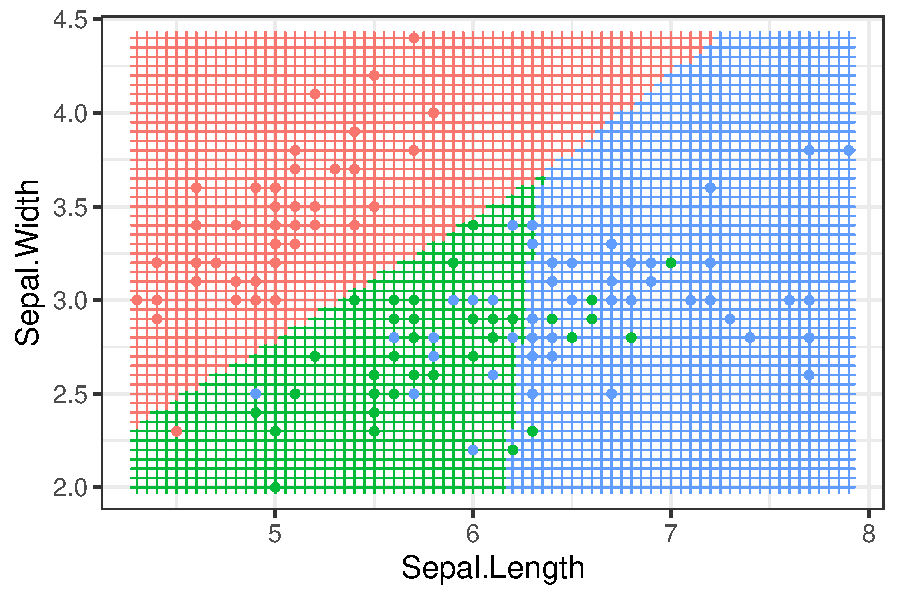
\includegraphics[width=\textwidth]{scripts/output/lda_regions.pdf}
      \caption{LDA classification regions.}
    \end{subfigure}
    \hfill
    \begin{subfigure}[b]{0.45\textwidth}
      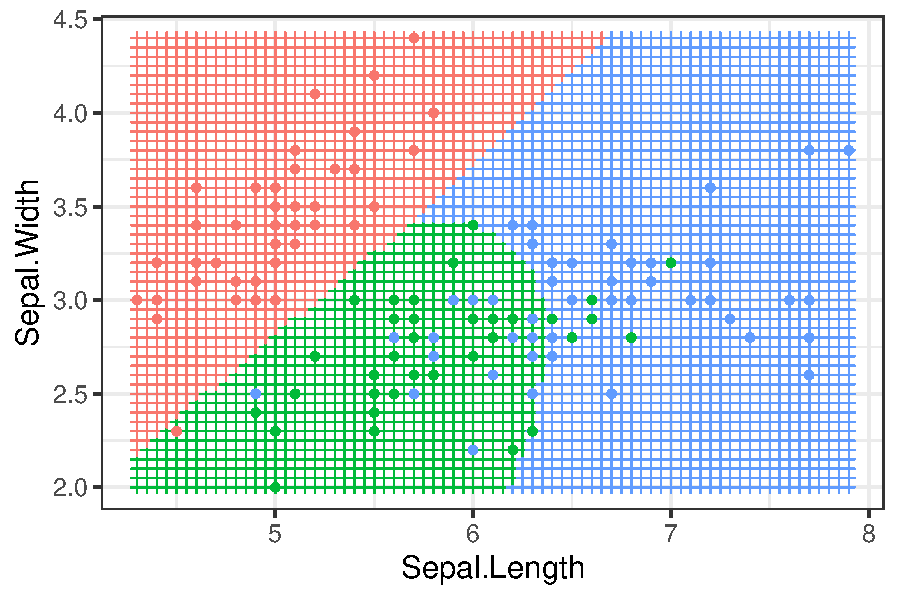
\includegraphics[width=\textwidth]{scripts/output/qda_regions.pdf}
      \caption{QDA classification regions.}
    \end{subfigure}
    \caption{Classification regions for LDA and QDA performed on the \textit{Iris} dataset, considering only the variables \textit{sepal width} and \textit{sepal length}.
    Note that the LDA boundaries are linear while QDA include a non-linear boundary.}
  \end{figure}
\end{frame}

\subsection{Naive Bayes}
\begin{frame}{\secname}{\subsecname}

\end{frame}

\section{Trees}

\subsection{Overview}
\begin{frame}{\secname}{\subsecname}

\end{frame}

\subsection{Introduction}
\begin{frame}{\secname}{\subsecname}
  Tree-based methods are supervised learning methods which can be used for both regression and classification.
  
  They work by segmenting the space into a number of simple regions and then, typically, use the mean of the region to make predictions.
  
  Because the segmentation of the space can be summarized in a tree, we call these methods tree-based.
\end{frame}

\subsection{Classification and Regression Trees (CART)}
\begin{frame}{\secname}{\subsecname}

\end{frame}

\subsection{Bagging}
\begin{frame}{\secname}{\subsecname}

\end{frame}

\subsection{Random Forest}
\begin{frame}{\secname}{\subsecname}

\end{frame}

\subsection{Boosting}
\begin{frame}{\secname}{\subsecname}

\end{frame}

\section{Support Vector Machines}

\subsection{Overview}
\begin{frame}{\secname}{\subsecname}
  
\end{frame}

\section{Neural Networks}

\subsection{Overview}
\begin{frame}{\secname}{\subsecname}
  
\end{frame}

\subsection{Perceptron}
\begin{frame}{\secname}{\subsecname}
    \textbf{Backpropagation}: For a given loss function $L$ we look for $\frac{\partial L}{\partial w_i}$.
    We start with initial values for the weights, which we shall denote $w_{old}$.
    Then we update the weights by $w_{new} = w_{old} - \eta \frac{\partial L}{\partial w}$.
    One iteration is called an \textbf{epoch}.
\end{frame}

{\aauwavesbg
\begin{frame}[plain,noframenumbering]
\end{frame}}
%%%%%%%%%%%%%%%%

\end{document}
